\documentclass[11pt]{article}
\usepackage[a4paper,left=20mm,top=10mm,bottom=25mm,right=20mm]{geometry}
\usepackage[OT2]{fontenc}
\usepackage{amsmath,amsfonts,amsthm}
\usepackage{hyperref}
\usepackage{pdfpages}

\newcommand\tsd{\theoremstyle{definition}}
\newcommand\tsr{\theoremstyle{remark}}
\newcommand\eng{\fontencoding{OT1}\fontfamily{\rmdefault}\selectfont}
\newcommand\srb{\fontencoding{OT2}\fontfamily{\rmdefault}\selectfont}

\pagenumbering{gobble}
\newlength\tindent
\setlength{\tindent}{\parindent}
\setlength{\parindent}{0pt}
\renewcommand{\indent}{\hspace*{\tindent}}

\title{\bf{Probijanje zvuchnog zida}}
\author{\Large Aleksa Vuchkovic1, 3c}
\date{}

\begin{document}
\maketitle
\large
\section{Uvod}
Zvuchni zid ili zvuchna barijera, fizichka pojava koja nastaje kada se poravnaju brzine izvora zvuka i zvuka i kada se u jednoj tachki dodiruju svi oscilujuc1i talasi zvuka i oscilujuc1i talasi izvora zvuka. U toj tachki je akumulirana maksimalna oscilatorna energija. Ta moc1na energet\/ska tachka se zove zvuchni zid ili zvuchna barijera.

\begin{center}
    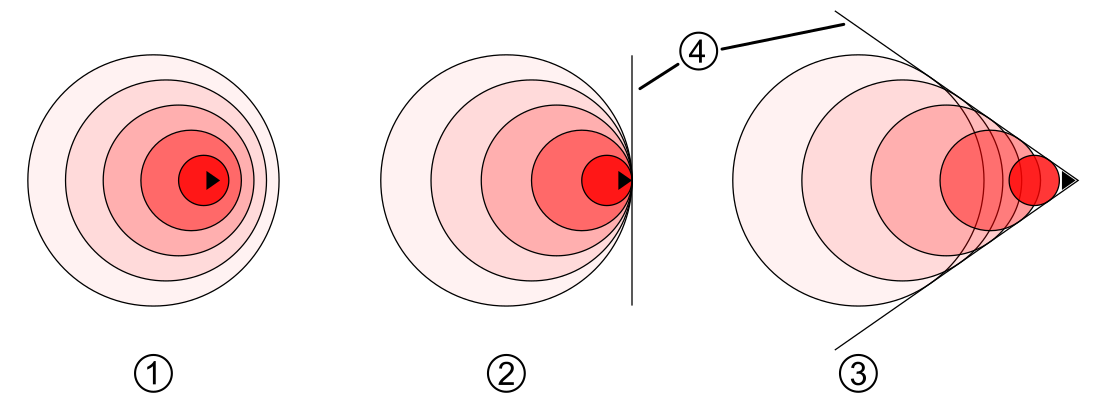
\includegraphics[scale=0.4]{Sound_barrier_chart.png}
\end{center}

\subsection{Doplerov efekat}
$\nu_L=\displaystyle\frac{u\pm u_L}{u\pm u_S}\cdot \nu_S$\\

U trenutku kad je brzina tela jednaka brzini zvuka primec1ujemo da je frekvencija primaoca beskonachna. Znachi da je, u tom delic1u vremena u kome su jednaki brzina zvuka i izvora (avion), frekvencija maksimalna, priblizhna beskonachnoj, pa otuda fatalno razorna.\\

\subsection{Mahov broj}
Mahov broj je odnos brzine kretanja tela i brzine prostiranja zvuka, izazvanog poremec1ajem, usled kretanja toga tela kroz fluid. Ovaj fenomen, dobio je naziv prema austrijskom fizicharu i filozofu Ernstu Mahu. Obelezhava se sa $M$.\\

Mahov broj je uveden u aerodinamiku, kao parametar, u cilju identifikacije uticaja stish\/ljivosti na karakteristike strujanja vazduha. Koristi se i shire, kao bezdimenzionziona fizichka velichina, u gasodinamici.

\newpage
\section{Primeri probijanja zvuchnog zida}
\subsection{Avionom}
Najchesh\/c1i, svakodnevni primer probijanja zvuchnog zida.\\

\textbf{Istorija:}\\
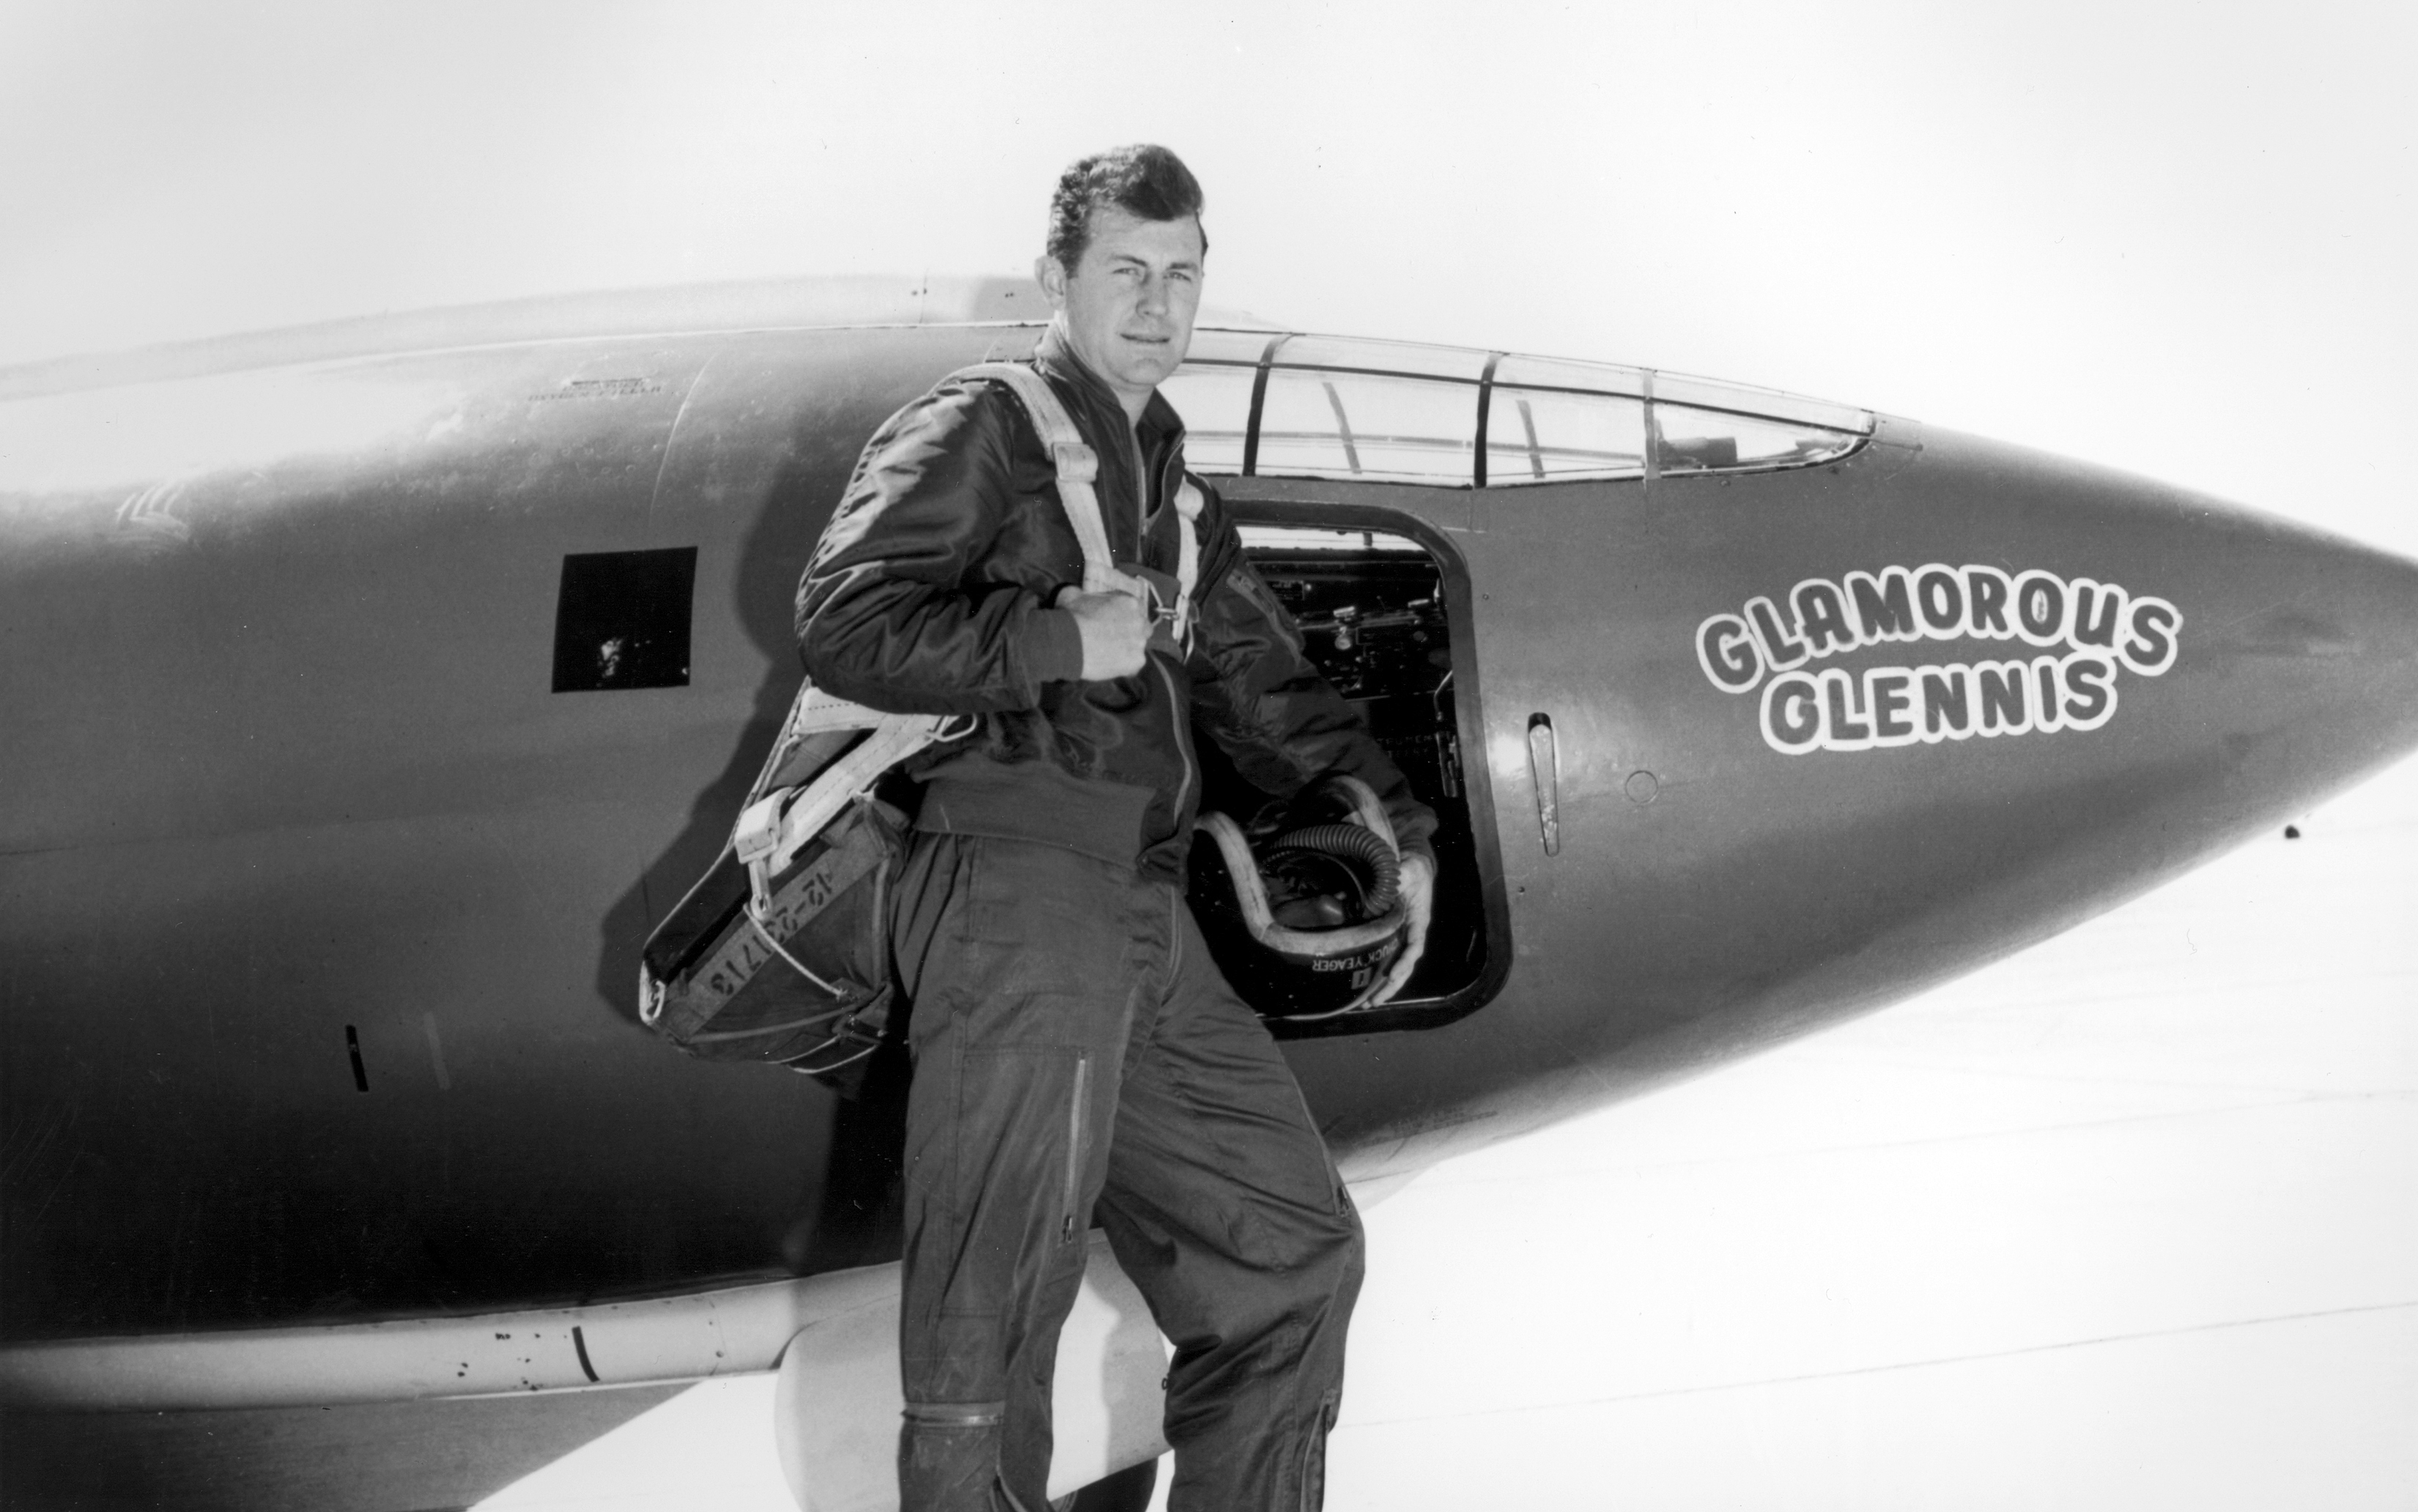
\includegraphics[scale=0.1]{Chuck_Yeager.jpg}
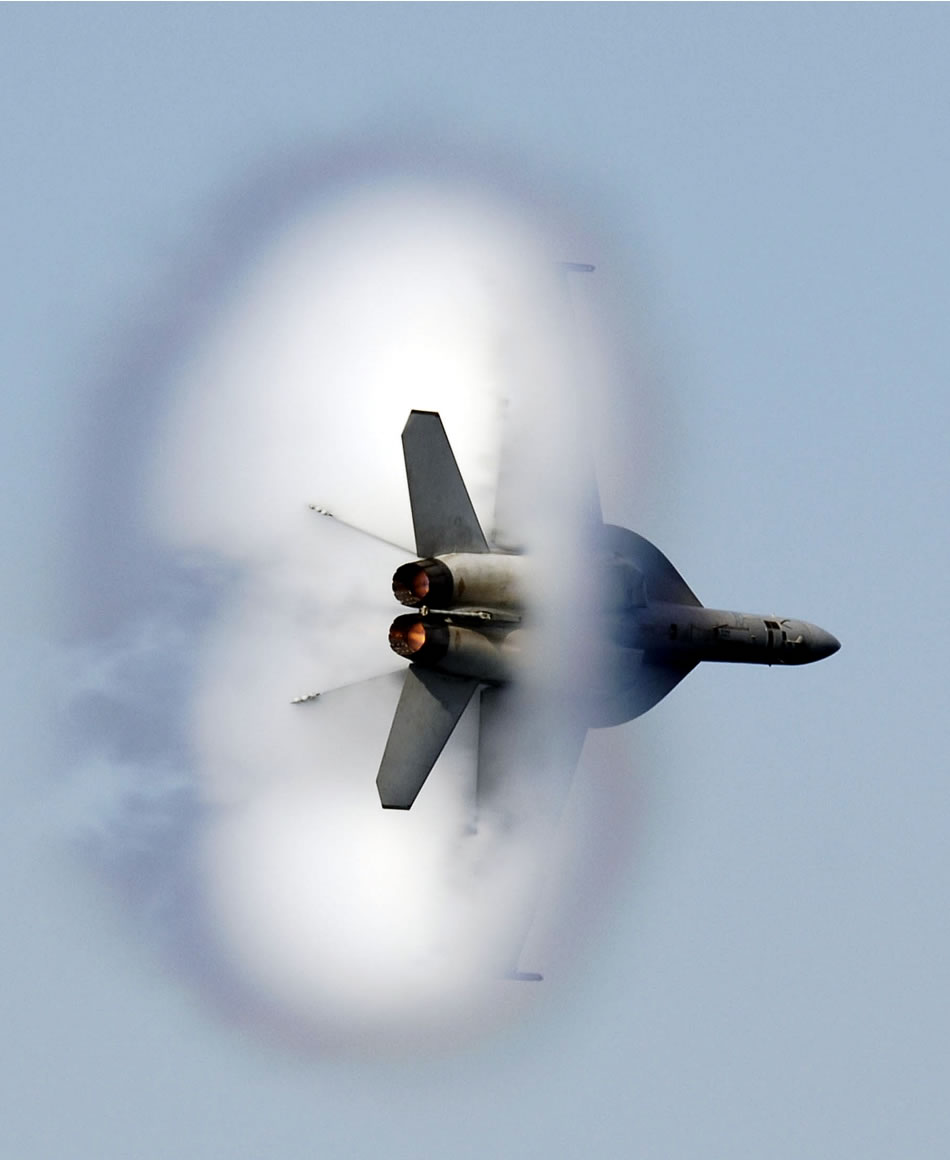
\includegraphics[scale=0.178]{F-18-diamondback_blast.jpg}\\
Prva slika: Chak Jegar ispred $Bell\ Ks-1$, prve letelice koja je probila zvuchnu barijeru u ravnom letu 14. oktobra 1947. godine\\
Druga slika: Brzo zgushnjavanje vodene pare zahvaljujuc1i probijanju zvuchnog zida koje se vidi slobodnim okom.\\

\textbf{Problem zvuchnog zida u konstrukciji aviona:}\\
Avion, sa moc1nim motorima koji ga pokrec1u, je i izvor snazhnih vibracija i oscilovanja chestica materijala od kojih je nachinjen. Ove vibracije pokrec1u chestice okolnog vazduha terajuc1i ih da i one osciluju i tako proizvode zvuk. Sada imamo, na jednoj strani, izvor zvuka (avion) i na drugoj, avinonov sopstveni zvuk. Izvor zvuka - avion, ima svoju brzinu. Proizvedeni oscilovani vazduh - zvuk, ima svoju brzinu od 340 metara u sekundi. Kada avion dostigne sopstveni zvuk, tj. kada im se brzine izjednache, dolazi do interferencije, slaganja-sabiranja amplituda oscilujuc1ih chestica aviona i oscilujuc1ih chestica vazduha - zvuka. Time se amplitude oscilujuc1ih chestica od kojih je sačinjen avion dupliraju.\\

\textbf{Reshenje problema:}\\
Kako tehnologija materijala za proizvodnju aviona nije u bliskoj buduc1nosti obec1avala materijale vec1ih chvrstina i odgovarajuc1u izdrzhljivost avionskih konstrukcija za tako velika oscilatorna opterec1enja, ostalo je samo da se poradi na materijalima i konstrukcijama koje c1e omoguc1iti povec1anja ubrzanja aviona. Tachnije, da se avion uchini toliko ubrzanim i moc1nim, da u najkrac1em moguc1em vremenu savlada i nadmashi brzinu sopstvengog zvuka. To je bio jedini nachin. Skrac1enje vremena boravka aviona u nivou brzine sopstvenog zvuka, omoguc1ilo je konachno savladavanje i probijanje te moc1ne prepreke - zvuchnog zida, i konachno ulazhenje u svet nadzvuchnog kretanja. 

\subsection{Raketom}
\eng\url{https://www.youtube.com/watch?v=q9S0z1ofcIc}\srb

\subsection{Automobilom}
$ThrustSSC$ drzhi svet\/ski rekord u kopnenoj brzini, postavljen 15. oktobra 1997, kada je postigao brzinu od 1.228$\frac{km}{h}$ i postao prvo kopneno vozilo koje je zvanichno probilo zvuchnu barijeru.\\

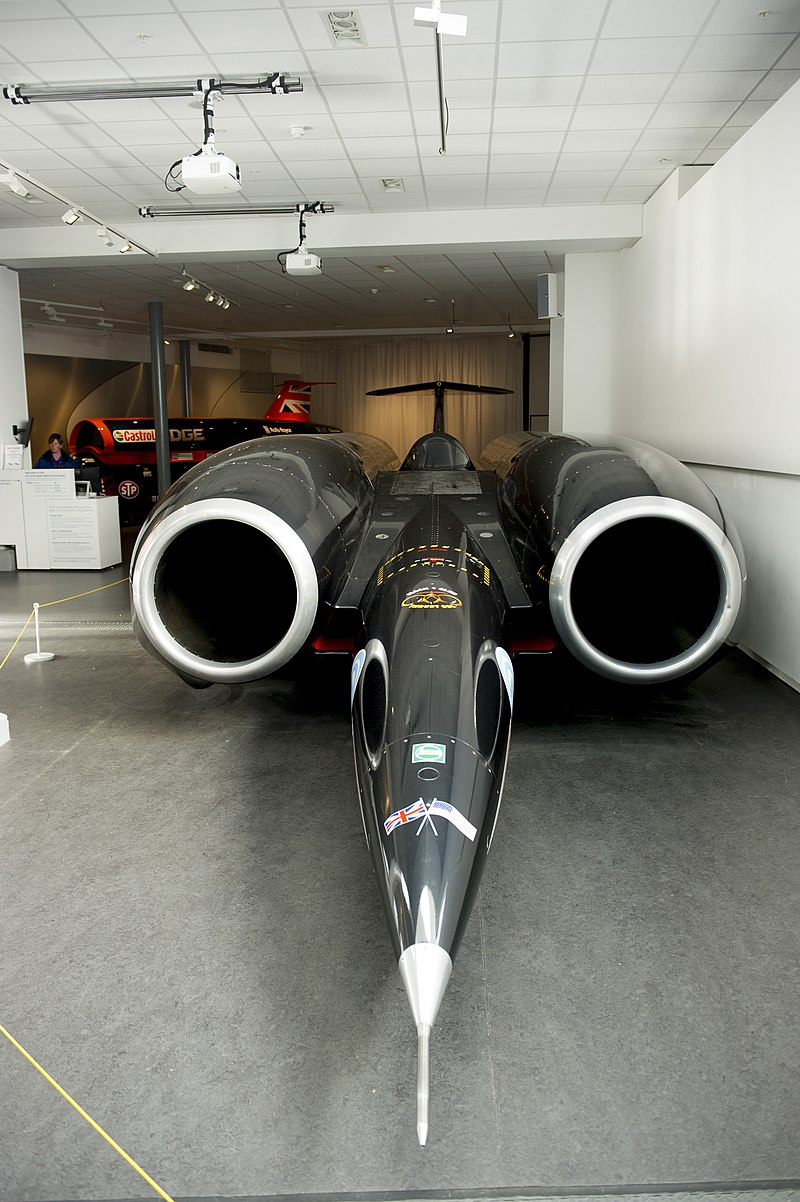
\includegraphics[scale=0.2]{Thrust_SSC.jpg}\hspace{1cm}
\includegraphics[scale=0.2]{BLOODHOUND_LSR_06.jpg}

\eng Thrust supersonic car(1997) \hspace{4.5cm} Bloodhunt LSR(2019)\srb\\

\eng\url{https://en.wikipedia.org/wiki/ThrustSSC}\srb\\
\eng\url{https://en.wikipedia.org/wiki/Bloodhound_LSR}\srb

\subsection{Vulkan probija zvuchni zid}
Planina Tavurvur u Papua Novoj Gvineji snimljena avgusta 2014. godine.\\
\eng\url{https://www.youtube.com/watch?v=BUREX8aFbMs}\srb

\subsection{Meteor probija zvuchni zid}
Buduc1i da meteori mogu pogoditi vrh atmosfere brzinom vec1om od 20000$\frac{km}{h}$, lako mogu probiti zvuchnu barijeru. Meteor se uglavnom raspadne pre nego shto padne na zemlju, ali uvek postoji verovatnoc1a da c1e neki manji fragmenti pogoditi zemlju ili vodu.\\
\eng\url{https://www.youtube.com/watch?v=_vqNiinWI7U}\srb

\subsection{Chovek u slobodnom padu}
14. oktobra 2012. godine je i prvi chovek van letelice, austrijski sportista Feliks Baumgartner, samo u primerenom letachkom kombinezonu-skafanderu, krec1uc1i se brzinama tela u slobodnom padu, probio zvuchni zid skochivshi iz kapsule balona sa visine od oko 39.000 metara. U njegovom poduhvatu je bilo nekoliko izuzetno rizichnih mesta. Pored zagrevanja skafandera usled trenja kroz atmosferu, znachajnih promena pritisaka i njihovog uskladjivanje u kapsuli i skafanderu sa spoljnim, veliko pitanje je bilo i kako c1e skakach proc1i u trenutku kada dostigne brzinu zvuka. Sigurno je da nije bilo velikog ubrzanja padobranca uslovljenog elementarnim zakonom fizike o telu u slobodnom padu, da Baumgartner ne bi prezhiveo ovaj skok. Kako je ubrzanje u slobodnom padu svakog tela vrlo veliko, tachnije, u ovom sluchaju dovoljno veliko, Baumgartner se spasonosno, u zanemarljivo kratkom vremenu kretao tom fatalnom brzinom zvuka.

\subsection{U vodi}
Frenk Heile, \eng P.h.D.\srb{} Fizika, Univerzitet Stanford:\\

"Da, probijanje zvuchnog zida c1e nastati ako objekat putuje vodom brzhe od brzine zvuka u vodi. Iako je voda relativno nestishljiva u poredjenju sa vazduhom, ona prenosi zvuchne talase i stoga c1e zaista imati konus u obliku zvuchnog zida koji se emituje sa prednje ivice bilo kog predmeta koji se krec1e kroz vodu brzhe od brzine zvuka. Pri $20^{\circ} C$ i pritisku od 1 $atm$, brzina zvuka u vazduhu je 343$\frac{m}{s}$ ili 1236$\frac{km}{h}$, dok je brzina zvuka u vodi je 1482$\frac{m}{s}$ ili 5336$\frac{km}{h}$, tako da je gotovo 4,5 puta brzhi nego u vazduhu.\\

Jedna razlika izmedju predmeta koji se krec1u vazduhom u odnosu na kretanje vodom je ta shto c1e, kada se u vodi predje brzina zvuka, doc1i do superkavitacije - postojac1e deo iza nosa objekta gde je pritisak vode ispod pritiska pare shto uzrokuje mehur pritiska pare koji se stvara iza predmeta. Ovo mozhe u velikoj meri smanjiti trenje kozhe predmeta jer c1e samo nos predmeta biti u kontaktu sa vodom."\\

\eng\url{https://www.reddit.com/r/askscience/comments/69kfdm/can_you_create_a_sonic_boom_underwater/}\srb

\end{document}